\section{Diagramme de Classes}

\begin{figure}[!ht]

\includegraphics[height=1.1\textwidth]{ClassesIntelliJ}
\centering
\caption{Diagramme de Classes Complet}
\label{uml:classes}
\end{figure}

\paragraph{Diagramme de classe:} le diagramme complet étant difficilement lisible, nous l'avons séparé en deux parties pour faciliter la lecture. 
Le diagramme complet est disponible sous format png dans doc/images/ClassesIntelliJ.png

\begin{figure}[!ht]
\includegraphics[width=1\textwidth]{ClassesHaut}
\centering
\caption{Diagramme de Classes partie du haut}
\label{uml:classes-haut}
\end{figure}


\paragraph{}
\begin{figure}[!ht]
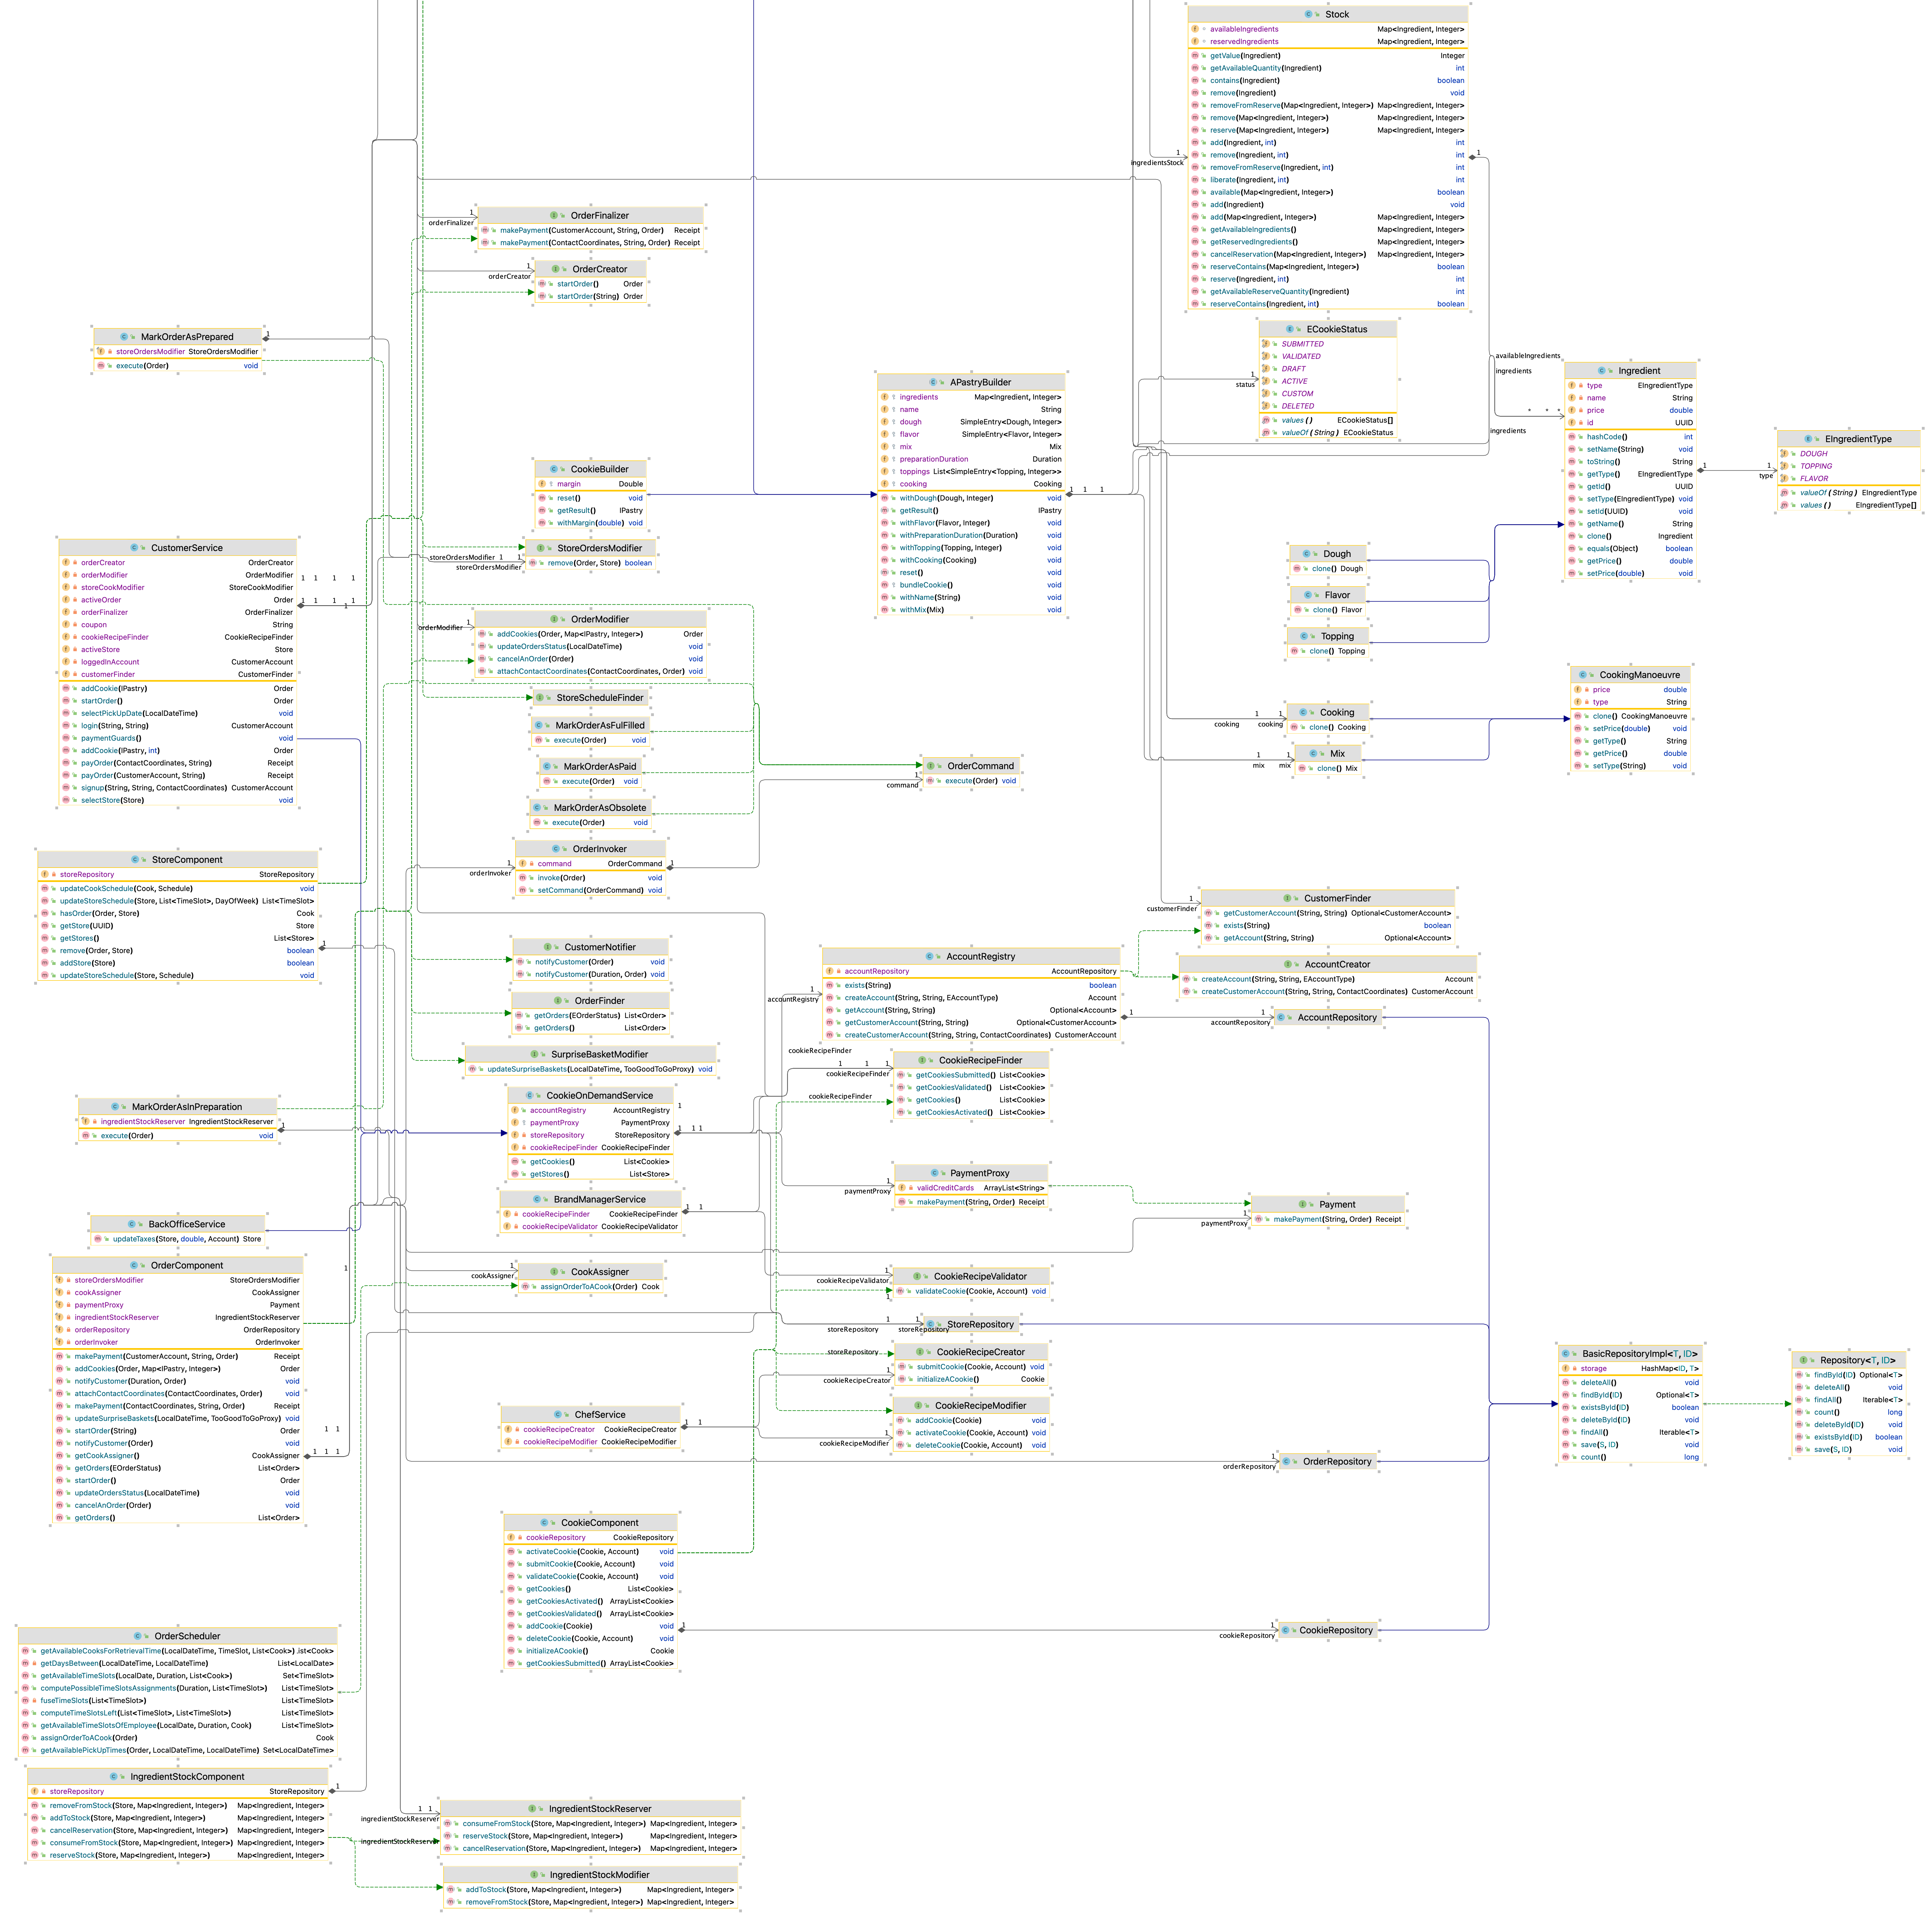
\includegraphics[width=1\textwidth]{ClassesBas}
\centering
\caption{Diagramme de Classes partie du bas}
\label{uml:classes-bas}
\end{figure}
